\documentclass[12pt]{article}
\usepackage{amssymb,amsmath}% http://ctan.org/pkg/{amssymb,amsmath}
\usepackage{braket}% http://ctan.org/pkg/braket
\usepackage[margin=0.1in]{geometry}
\usepackage{graphicx}
\usepackage{subcaption}
\begin{document}





\[\text{\bf{Customer C Spend on Order X}} = c*r*t + \epsilon \]
\[c = \text{Customer's mean order amount in dollars where } c \sim \mathcal{N}(\$100,\$25).\]
\[r = \text{Scalar corresponding to mean retailer order amount where } r \sim \mathcal{N}(1.0,0.05).\]
\[t = \text{Whether or not the customer recieved the experimental treatment } t \in [1,1.1].\]
\[\epsilon = \text{Random noise where } \epsilon \sim \mathcal{N}(\$10,\$1).\]
\\
\indent\indent Recall that the data is clustered (we aspire for customers to place multiple orders!), thus:
\[\text{The number of orders placed by Customer C }  \sim exp(\lambda = 1).\]



\noindent
\begin{figure}[b]
\centering
\begin{subfigure}{.32\textwidth}
    \centering
    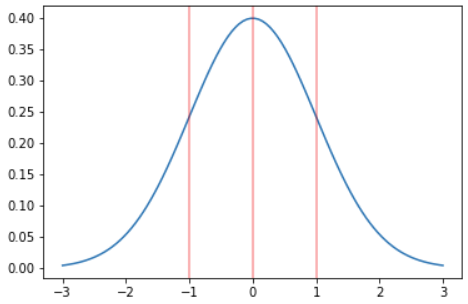
\includegraphics[width=0.75\textwidth]{sd_3.png}
    \caption[short]{$\mu$ +/- [1]$\sigma$ \\with 500 iterations.}
    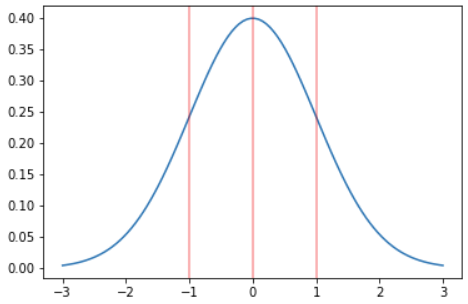
\includegraphics[width=0.75\textwidth]{sd_3.png}
    \caption[short]{$\mu$ +/- [1,2]$\sigma$ \\with 500 iterations.}
    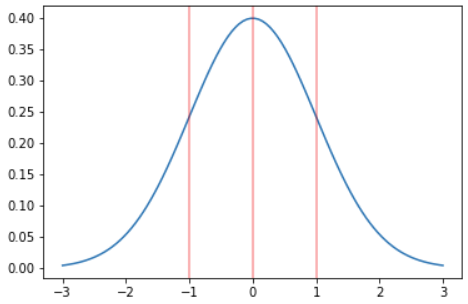
\includegraphics[width=0.75\textwidth]{sd_3.png}
    \caption[short]{$\mu$ +/- [1,2,3]$\sigma$ \\with 500 iterations.}
\end{subfigure}
\begin{subfigure}{.32\textwidth}
    \centering
    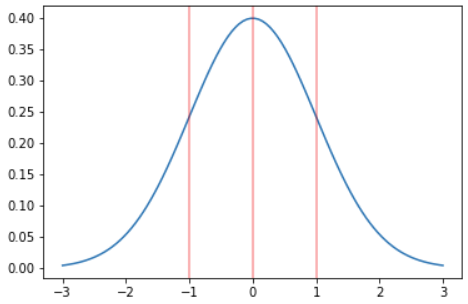
\includegraphics[width=0.75\textwidth]{sd_3.png}
    \caption[short]{$\mu$ +/- [1]$\sigma$ \\with 1,000 iterations.}
    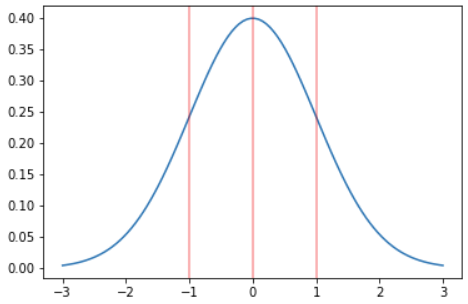
\includegraphics[width=0.75\textwidth]{sd_3.png}
    \caption[short]{$\mu$ +/- [1,2]$\sigma$ \\with 1,000 iterations.}
    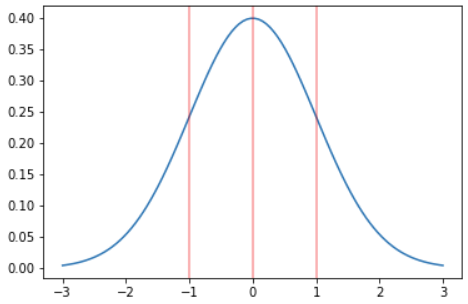
\includegraphics[width=0.75\textwidth]{sd_3.png}
    \caption[short]{$\mu$ +/- [1,2,3]$\sigma$ \\with 1,000 iterations.}
\end{subfigure}
\begin{subfigure}{.32\textwidth}
    \centering
    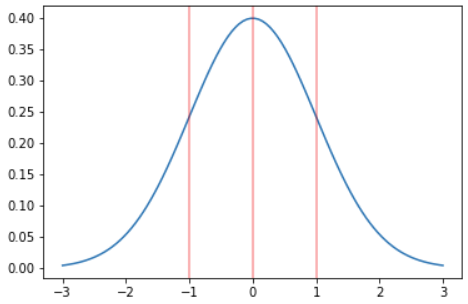
\includegraphics[width=0.75\textwidth]{sd_3.png}
    \caption[short]{$\mu$ +/- [1]$\sigma$ \\with 2,000 iterations.}
    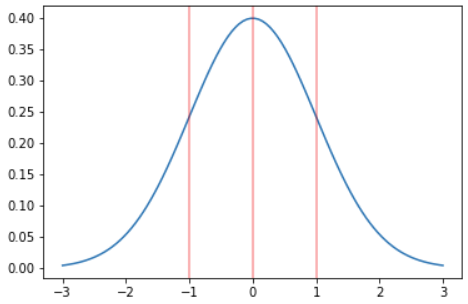
\includegraphics[width=0.75\textwidth]{sd_3.png}
    \caption[short]{$\mu$ +/- [1,2]$\sigma$ \\with 2,000 iterations.}
    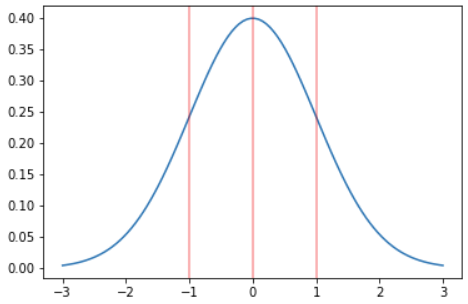
\includegraphics[width=0.75\textwidth]{sd_3.png}
    \caption[short]{$\mu$ +/- [1,2,3]$\sigma$ \\with 2,000 iterations.}
\end{subfigure}%
\caption[short]{}
\end{figure}

\end{document}